\documentclass{beamer}

\usetheme{simple}

\newcommand{\emojipizza}{
\includegraphics{img/pizza.png}}

\usepackage{caption}
\usepackage{xcolor}
\usepackage{fancyvrb}
\usepackage{ulem}
\usetikzlibrary{positioning,calc,automata}

\title{CSC363 Tutorial \#4}
\subtitle{Turing reductions! (and some assignment feedback)}
\date{February 09, 2022}
\institute{}

\newcommand{\N}{\mathbb N}

\setwatermark{
\includegraphics[height=8cm]{img/chungus.png}}

\begin{document}

\maketitle

\begin{frame}{Learning objectives this tutorial}
\begin{itemize}
\item Review (hopefully, if you remember) Turing reductions.
\item Learn (or review, if you've attended the Monday lecture) $m$-reductions and $1$-reductions.
\item Distinguish between Turing reductions, $m$-reductions, and $1$-reductions.
\end{itemize}
\end{frame}

\begin{frame}{Assignment 1 stuff}
Assignment 1 feedback has been posted to Pizza. \emojipizza

Please read through it! Some common mistakes throughout (also appearing on Assignment 2):

\pause


\begin{itemize}
    \item Given a CE set $S$, we might not be able to determine if an arbitrary $x \in \N$ is in $S$ or not (unless we can assume $S$ is computable). The best we can do is confirm that $x \in S$, and loop otherwise (by printing out elements of $S$ until we find $x$). Thus, some condition like ``if $x \in S$'' might cause your program to get stuck.
    
    \pause
    
    \begin{figure}[h]
        \centering
        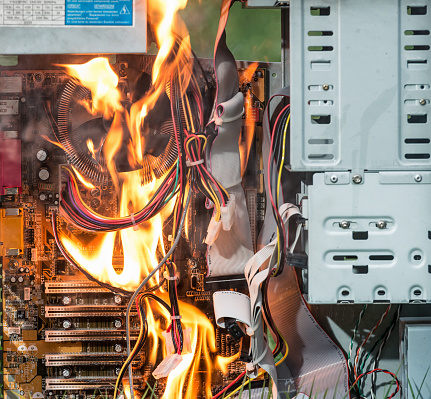
\includegraphics[scale=0.8]{img/computer_fire.jpg}
    \end{figure}
    
    \item Sometimes, the solution proves a completely different (and maybe more trivial) statement. Make sure to reiterate what you are trying to prove, so that you don't lose track!
\end{itemize}
\end{frame}


\begin{frame}{Turing reductions!}
\only<1>{
\textbf{Task:} Show that $K = \{x: \varphi_x(x)\text{ halts} \}$ is computable!
}
\only<2->{
\sout{\textbf{Task:} Show that $K = \{x: \varphi_x(x)\text{ halts} \}$ is computable!}
}

\pause

\textbf{Ans:} That's kinda impossible...

\pause

But what if some person comes along and gives you this \textbf{black box} (or \textbf{oracle}) that tells you whether something is in $K$? \tiny{This would probably break some law of the universe, but still}
\begin{figure}[h]
    \centering
    
\includegraphics[scale=0.4]{img/eminem.jpg}
\end{figure}

\end{frame}

\begin{frame}{Turing reductions!}
But what if some person comes along and gives you this \textbf{black box} (or \textbf{oracle}) that tells you whether something is in $K$?
\begin{figure}[h]
    \centering
    
\includegraphics[scale=0.2]{img/eminem.jpg}
\end{figure}

Is $K$ now computable? \pause Yes, because now we can check if something is in $K$ or not by just feeding it into this black box. \pause

What about $\bar{K}$? Without Eminem's help, $\bar{K}$ is not even CE. Is it now computable? \pause Yes, because we can again use this box to determine if something is in $\bar{K}$ (so not in $K$) or not.

\end{frame}

\begin{frame}{Turing reductions!}
If we can compute (the indicator of) $K$, then we can compute $\bar{K}$. So in some sense, $K$ is \textit{at least as hard to compute} as $K$: once we are able to compute $K$, we will also be able to compute $\bar{K}$. We can \textit{reduce} the problem of computing $\bar{K}$ to the problem of computing $K$.

\begin{figure}[h]
    \centering
    
\includegraphics[scale=0.2]{img/eminem.jpg}
\end{figure}

\pause

\textbf{Definition:} Let $A, B \subseteq \N$ be sets. We say that \textbf{$A$ Turing reduces to $B$}, written $A \leq_T B$, if we can compute $A$ given a black box for $B$.

\vspace{2mm}

\pause

You may think of $A \leq_T B$ as saying ``$A$ is less difficult than $B$'', in that we can reduce the problem of computing $A$ into the problem of computing $B$.

\end{frame}

\begin{frame}{Turing reductions!}
\textbf{Definition:} Let $A, B \subseteq \N$ be sets. We say that \textbf{$A$ Turing reduces to $B$}, written $A \leq_T B$, if we can compute $A$ given a black box for $B$.

\vspace{2mm}

\textbf{Task:} Let $S$ be a computable set. Briefly explain why $S \leq_T K$.

\pause

\textbf{Ans:} Since $S$ is computable, given a black box for $K$, we can just throw away the black box and compute $S$ directly!
\begin{figure}[h]
    \centering
    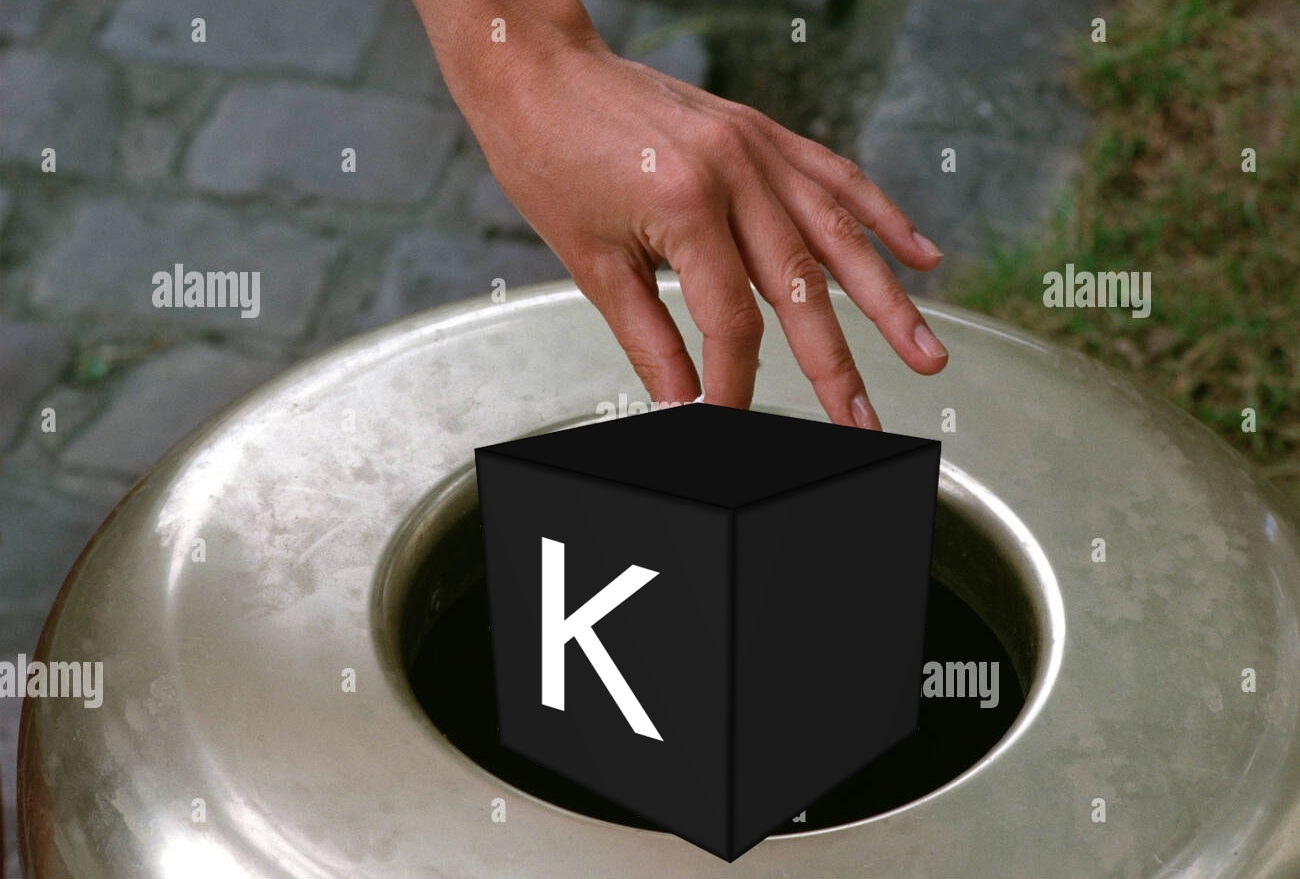
\includegraphics[scale=0.5]{img/trash.jpg}
\end{figure}

\end{frame}

\begin{frame}[fragile]{Turing reductions!}
\textbf{Definition:} Let $A, B \subseteq \N$ be sets. We say that \textbf{$A$ Turing reduces to $B$}, written $A \leq_T B$, if we can compute $A$ given a black box for $B$.

\vspace{2mm}

\textbf{Task:} Let $K = \{x: \phi_x(x) \text{ halts}\}$, and 
$$H = \{(x, e): \phi_e(x) \text{ halts}\}.$$
Show that $K \leq_T H$.

\pause

\textbf{Ans:} Given a black box for $H$, we can compute $K$ using the following procedure:
\begin{verbatim}
def is_in_K(x):
  if (x, x) in H:
    return True
  else: return False
\end{verbatim}

\end{frame}

\begin{frame}[fragile]{Turing reductions!}
\textbf{Task:} Let $K = \{x: \phi_x(x) \text{ halts}\}$, and $H = \{(x, e): \phi_e(x) \text{ halts}\}$.
Show that $H \leq_T K$. This is a bit trickier!

\pause

\vspace{2mm}

\textbf{Ans:} Given a black box for $K$, we can compute $H$ using the following procedure:
\begin{verbatim}
def is_in_H(x, e):
  Construct the TM M that does the following:
    M(y):
      (ignore y)
      Run the eth Turing machine on x
      Return if it halts
  Let z be the Turing Machine # of M
  if z in K:
    return True
  else: return False
\end{verbatim}

Notice: We construct $M$, but we don't actually run it! Running $M$ might result in a loop.

\end{frame}

\begin{frame}{Turing reductions!}
\textbf{Definition:} If $A \leq_T B$ and $B \leq_T A$, we say that \textbf{$A$ is Turing equivalent to $B$}, and write $A =_T B$.

\vspace{2mm}

In some sense, this says $A$ is equivalent in computational difficulty to $B$: if we can compute one, then we can also compute the other.
\end{frame}

\begin{frame}{$m$-reductions...}

We'll introduce another reduction mechanism, called an $m$-reduction.

\textbf{Definition:} Let $A, B$ be sets. We say that $A \leq_m B$ if there exists a \textit{computable} function $f$ such that 
$$x \in A \Leftrightarrow f(x) \in B.$$

\begin{figure}[h]
    \centering
    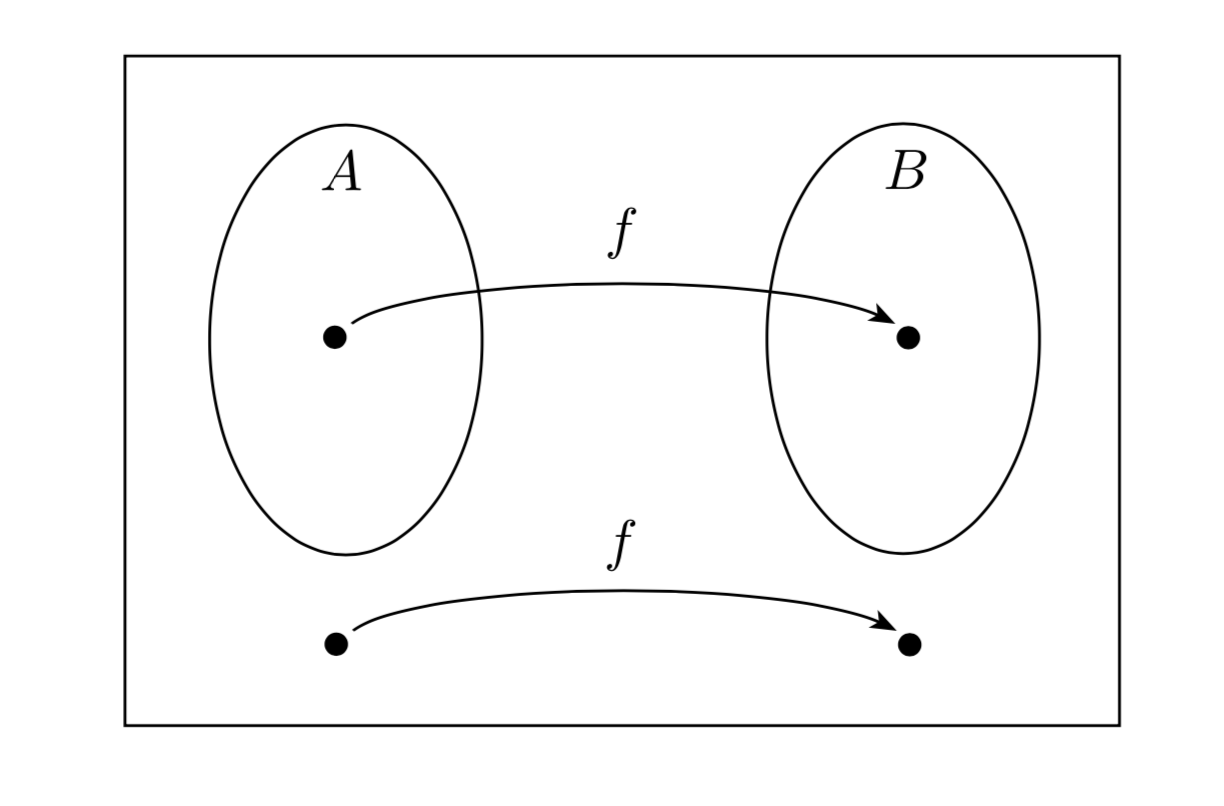
\includegraphics[scale=0.3]{img/mapping_reduc.png}
    \caption*{\tiny{stolen from \url{https://liyanxu.blog/2019/05/06/mapping-reducibility-turing-reducibility-kolmogorov-complexity/}}}
\end{figure}

\end{frame}

\begin{frame}{$m$-reductions...}

\textbf{Definition:} Let $A, B$ be sets. We say that $A \leq_m B$ if there exists a \textit{computable} function $f$ such that 
$$x \in A \Leftrightarrow f(x) \in B.$$

\vspace{2mm}

It turns out that $m$-reduction is stronger than Turing reduction: if $A \leq_m B$, then $A \leq_T B$. However, there do exists sets $A, B$ such that $A \leq_T B$ but not $A \leq_m B$.

\pause
\vspace{2mm}

\textbf{Task:} Show that if $A \leq_m B$, then $A \leq_T B$. \textit{Hint: Write out the meaning of each of those definitions.}

\end{frame}

\begin{frame}[fragile]{$m$-reductions...}

\textbf{Definition:} Let $A, B$ be sets. We say that $A \leq_m B$ if there exists a \textit{computable} function $f$ such that 
$$x \in A \Leftrightarrow f(x) \in B.$$

\textbf{Task:} Show that if $A \leq_m B$, then $A \leq_T B$. \textit{Hint: Write out the meaning of each of those definitions.}

\textbf{Ans:} Suppose $A \leq_m B$. Then there exists a computable function $f$ such that
$$x \in A \Leftrightarrow f(x) \in B.$$
To show $A \leq_T B$, suppose we are given a black box for $B$. We can compute $A$ as follows:
\begin{verbatim}
def is_in_A(x):
  return True if f(x) in B, False otherwise.
\end{verbatim}

\end{frame}

\begin{frame}[fragile]{$m$-reductions...}

\textbf{Task:} Show that $\emptyset \leq_T \N$, but not $\emptyset \leq_m \N$.

\pause

\textbf{Ans:} $\emptyset$ is computable, so we automatically get $\emptyset \leq_T \N$ by just tossing away the black box for $\N$. However, there is no computable function $f$ such that $$x \in \emptyset \Leftrightarrow f(x) \in \N.$$
This is because there isn't even any function $f$ that satisfies the above, regardless of computability of $f$! (Why?)

\end{frame}


\begin{frame}[fragile]{$m$-reductions...}

So what we have just shown is that $A \leq_m B \Rightarrow A \leq_T B$, but $A \leq_T B \not \Rightarrow A \leq_m B$. Thus, we may show Turing reducibility by showing $m$-reducibility, but not necessarily the other way around.

\vspace{2mm}

\pause

\textbf{Task:} Let $S \subseteq \N$ be computable, and $T \subseteq \N$ be any arbitrary set satisfying $T \neq \emptyset$ and $T \neq \N$. Show that $S \leq_m T$.

\pause

\vspace{2mm}

\textbf{Ans:} Since $T \neq \emptyset$, there is some $p \in T$. Since $T \neq \N$, there is some $q \in \N, q \notin T$. Define $f$ by
$$f(x) = \begin{cases}
p & x \in S\\
q & x \notin S.\\
\end{cases}$$
Since $S$ is computable, so is $f$. Furthermore, $x \in S \Leftrightarrow f(x) \in T$.

\end{frame}






\end{document}